
\documentclass{article}
\usepackage{eurosym}
\usepackage{graphicx}

\newcommand{\ether}{$\Xi$}
\newcommand{\ors}{{\sf ORS}}
\newcommand{\orsT}{{\sf ORS Token}}

\title{ORS Token Sale Smart Contracts}
%\author{L. Cremer, G. Baecker, S. Joergens}
\author{SICOS}
\date{May 12, 2018 - internal use only} 
 
\begin{document}

\maketitle


 \begin{abstract}
 Latest changes to contract specifications of the ORS tokensale during audit
 phase.\\\\
 The ORS tokensale contains of two smart contracts. The token contract is an standard contract from the Open
 Zeppelin library. The token sale contract is minting tokens directly to the
 addresses of the investors. There will be a KYC process done by an KYC service
 provider with an integrated KYCBase interface. Also an ICOEngineInterface
 provides informational functions for the Eidoo wallet.
 \end{abstract}

\section{Token Contract}
The token contract implements a ERC20 standard token. It is named \orsT.
Ticker symbol will be \ors. The number of decimals will be 18 to keep the
\ors \ resolution  identical to \ether. \\\\
The token contract emits the standard ERC20 events including a transfer event to
address 0x0 in case of issued tokens.\\\\
We rely on the broadly trusted Open
Zeppelin \footnote{https://github.com/OpenZeppelin/openzeppelin-solidity/tree/master/contracts/token}
implementation of an ERC20 compliant Token. The following extensions are used:

\subsection{Capped and Mintable}
Tokens are minted on demand by the owner of the token contract. Therefore the
ownership of the token contract has to be transfered to the token sale contract. The minting of tokens is capped at
$833,333,333$.

\subsection{Pausable}
Transfer of tokens is paused on construction of the token contract. Transfer of
tokens is unpaused on finalization of the token sale contract. No transfer of
tokens is possible during the ICO.

\subsection{Owned}
Minting and pausing functions are restricted to the token contract owner. The
ownership of the token contract is transfered to the token sale contract immediately after deploy.
\subsection{StandardBurnable}
Token can be irreversibly burned (destroyed) by the token holder at any time.

\section{Token Sale Contract}
The token sale contracts implements the Eidoo 
ICOEngineInterface
\footnote{https://github.com/eidoo/icoengine/blob/master/contracts/ICOEngineInterface.sol} 
 to provide the Eidoo app with informations on the ICO status.\\\\ 
 The token sale contract provides a function that enables the token contract owner to set the \orsT \ price at any time. 
 The price represents the \ors  \ per \ether \ rate. With a target price of
 $0.05$ \euro \ per \ors \ we will have a rate of $\approx 13,000$ according to
 a  price of $\approx 650$ \euro \ per \ether. \\\\ Tokens are issued
 immediatly within the transaction receiving the \ether \ payment.
\\\\
\noindent
Tokens are minted from different pools in the token sale contract. Any try to
mint tokens from an empty pool will revert the whole transaction. 

\begin{center}
\begin{table}[h]
\begin{tabular}{l|c|r|c}


Pool & & Cap & Drained \\\hline
Presale & $P$ &222,247,844& any time before finalization\\
Main ICO & $M$ &281,945,791&between start  and end date if ICO\\
Bonus & $B$ & 60,266,365& together with $M$ and at finalization\\
Team &  $T$ & 83,333,333& at finalization \\
Company &  $C$ & 127,206,667& at finalization\\
Advisors &  $A$ & 58,333,333& at finalization\\\hline
&&833,333,333&\\
\end{tabular}
\end{table}
\end{center}
%With $|M| + |P| = 500,000,000$.\\\\
%\noindent
The token sale consists of the three stages main ICO, presale and finalization:
\subsection{Main ICO}
The Main ICO starts at 2018-05-14T09:00:00+02:00 Unix timestamp
1526281200 and ends at
2018-05-26T23:00:00+02:00 Unix timestamp 1527368400. There may be an early end
if $|M| = 0$.
\\\\ Issued tokens are taken from $M$. Additional 5 \% bonus tokens are taken
from $B$ if the KYC is signed by the Eidoo Wallet. Requirement for the sizes of
$M$ and $B$ is:
\begin{eqnarray}
  |B| & \geq & \frac{|M|}{20} 
  \end{eqnarray}
When the cap of $M$ is
reached, the last investor will get the last tokens and the remaining \ether \
will be refunded.
Remaining tokens in $M$ after the end of the ICO will not be issued at all.
\subsection{Presale}
At any time before finalization tokens are issued to
presale investors by the owner of the token sale contract according to a list
provided by ORS. Bonus tokens issued to presale investors are added to the token
amount off-chain. Issued Tokens are taken from $P$.
The list contains the amounts of tokens
assigned to presale buyer addresses and complies to the choosen cap of
$P$. Let $(a_i,p_i)$ be the presale list entry issuing $p_i$ tokens to address $a_i$.
Requirement for the list with size $n$
is
\begin{eqnarray}
     |P| & = & \sum_{i=1}^n  p_i 
  \end{eqnarray}
because $|P| = 0$ is a precondition for finalization of the token sale contract.


\subsection{Finalization}
After end of main ICO and completness of  presale the
finalization stage takes place. $|T|+|C|$ tokens are issued to company wallet.
$|A|$ tokens are issued to advisors wallet. Remaining $|B|$ tokens are issued to
bounty wallet. Further miniting of tokens in token contract is disabled.
Transfers are unpaused in token contract. The ownership of the token contract is not
transferred. The token sale contract is useless from now on. The token contract
has no owner capable of acting.
\subsection{KYC}
The token sale contract implements the Eidoo KYCBase
\footnote{https://github.com/eidoo/icoengine/blob/master/contracts/KYCBase.sol}
(ors-integration branch) contract. Eidoo provides two addresses of KYC signers.
The first belongs to Eidoo wallet investors and will provide 5 \% bonus tokens. The second address belongs to all investors using Eidoo without the wallet. \\\\


\newpage


\section{Timeline}

\begin{center}
\begin{table}[h]
\begin{tabular}{r|l}

Date & Event \\\hline
$\approx$ 2018-05-11&Token contract deployment \\
&Token sale contract deployment \\
&Transfer of token contract ownership to token sale contract \\
&Etherscan code verification \\
&Transfer of ownership of token sale contract to \ors\\
& Issuing of presale tokens start\\
2018-05-14& Main ICO start\\
$<=$ 2018-05-26& Main ICO end\\
$\approx$ 2018-05-27& Finalization of token sale contract\\
& ERC20 transfers enabled\\

\end{tabular}
\end{table}
\end{center}


\section{Deployment Requirements}
The following requirements have to be fulfilled at deployment time 2018-05-11:
\begin{center}
\begin{table}[h]
\begin{tabular}{r|l|l}

Requirement & Source &Value\\\hline
Size of $P$ and $M$&\ors&see above \\
Initial token sale contract
owner&SICOS&\tt 0x6aA5a27132f2A828350e06Fb20e04e7E5e205e9A\\
Main ICO wallet&\ors&\tt 0xF5A4cD4E156170281880B645C2c36e4Da5610284\\
Bounty wallet&\ors&\tt0x6265D03b984C3e1378e42B132D2D76F5A1ccb9fF\\
Advisors wallet&\ors&\tt 0x43C954E971DB80573861baf0BDfCac1F69f8C0D5\\
Company wallet&\ors&\tt 0xF83547c41DBf888DA26d6e3F4A8C0dbA30134672\\
Eidoo wallet signer address&Eidoo&\tt 0xdd5ecefcaa0cb5d75f7b72dc9d2ce446d6d00520\\
Second signer address&Eidoo&\tt 0x4e315e5de2abbf7b745d9628ee60e4355c0fab86\\

\end{tabular}
\end{table}
\end{center}



\begin{figure}[!ht]
%\centering
  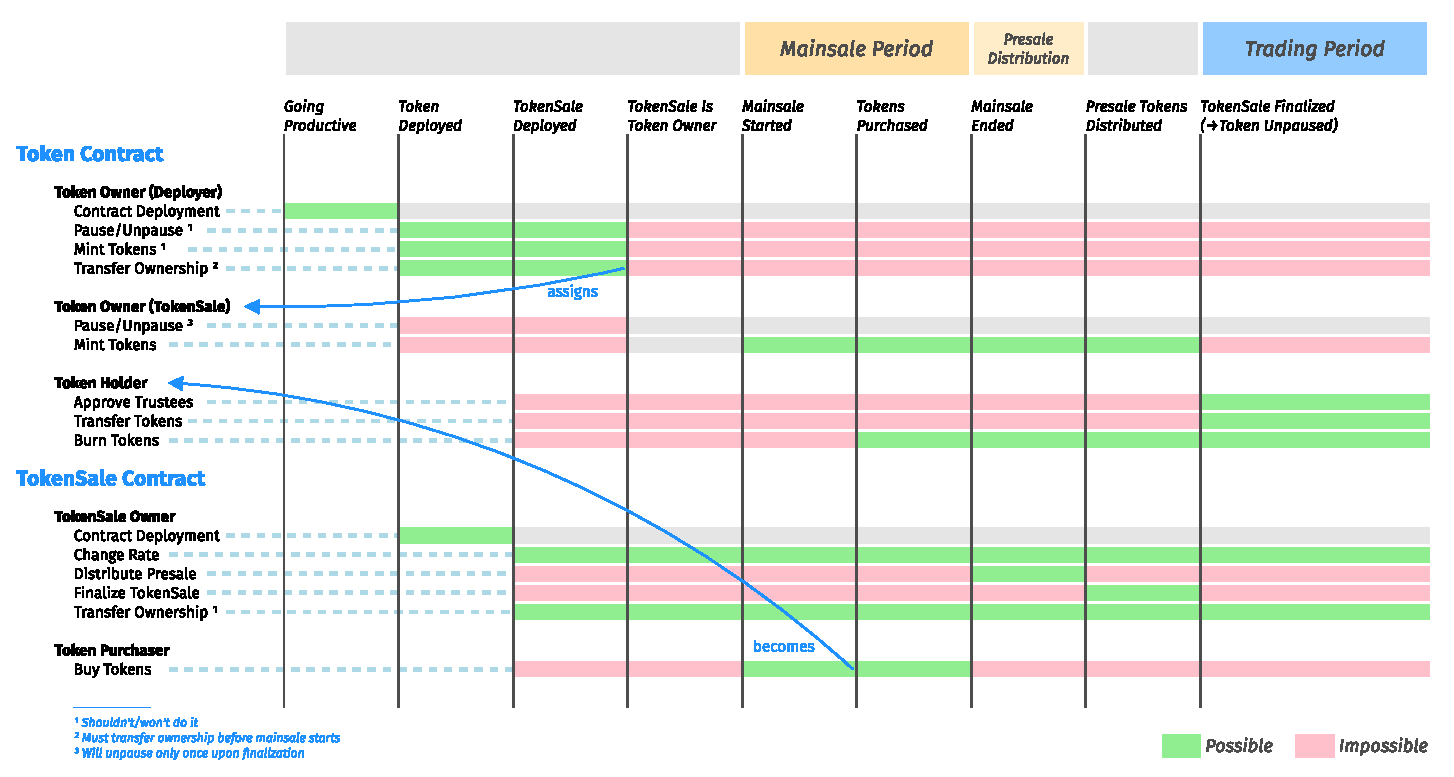
\includegraphics[width=1.7\textwidth,angle=90]{lifecycle.eps}

\end{figure}



%\bibliography{literatur}
\end{document}
